\documentclass[12pt, twoside]{article}
\usepackage[letterpaper, margin=1in, headsep=0.2in]{geometry}
\setlength{\headheight}{0.6in}
%\usepackage[english]{babel}
\usepackage[utf8]{inputenc}
\usepackage{microtype}
\usepackage{amsmath}
\usepackage{amssymb}
%\usepackage{amsfonts}
\usepackage{siunitx} %units in math. eg 20\milli\meter
\usepackage{yhmath} % for arcs, overparenth command
\usepackage{tikz} %graphics
\usetikzlibrary{quotes, angles}
\usepackage{graphicx} %consider setting \graphicspath{{images/}}
\usepackage{parskip} %no paragraph indent
\usepackage{enumitem}
\usepackage{multicol}
\usepackage{venndiagram}

\usepackage{fancyhdr}
\pagestyle{fancy}
\fancyhf{}
\renewcommand{\headrulewidth}{0pt} % disable the underline of the header
\raggedbottom
\hfuzz=2mm %suppresses overfull box warnings

\usepackage{hyperref}

\fancyhead[LE]{\thepage}
\fancyhead[RO]{\thepage \\ Name: \hspace{4cm} \,\\}
\fancyhead[LO]{BECA / Dr. Huson / Geometry\\*  Unit 6: Analytic geometry\\* 30 November 2022}

\begin{document}

\subsubsection*{6.6 Homework: Distance formula, perpendicular and parallel slopes}
\begin{enumerate}
  \item Graph and label the two equations. Mark their intersection as an ordered pair.

  \begin{multicols}{2}
    $y = -4x-6$ \\
    $x-3y = -21$
  \end{multicols}  \vspace{1cm}
  Are the lines parallel, perpendicular, or neither? Justify your answer.
  \vspace{1.5cm}

  \begin{center} %4 quadrant regents grid w T-Chart
  \begin{tikzpicture}[scale=.635]
    \draw [help lines] (-10,-8) grid (10,10);
    \draw [thick, ->] (-10.2,0) -- (10.4,0) node [below right] {$x$};
    \draw [thick, ->] (0,-8.2)--(0,10.4) node [left] {$y$};
  \end{tikzpicture}
  \end{center}

\item The line $l$ has the equation $y= 3x+2$.
\begin{enumerate}
  \item What is the slope of the line $k$, given $k \parallel l$?
  \vspace{1cm}
  \item What is the slope of the line $m$, given $m \perp l$?
  \vspace{1cm}
\end{enumerate}

\newpage
\item On the graph below, draw $\overline{AB}$, with $A(-1,1)$ and $B(7,3)$, labeling the end points. Determine and state the coordinates of the midpoint $M$ of $\overline{AB}$ and mark and label it on the graph.\\
\begin{tikzpicture}[scale=.635]
  \draw [help lines] (-3,-2) grid (8,6);
  \draw [thick, ->] (-3.2,0) -- (8.4,0) node [below right] {$x$};
  \draw [thick, ->] (0,-2.2)--(0,6.4) node [left] {$y$};
\end{tikzpicture}

\item $A(-1,7)$ is one endpoint of $\overline{AB}$. The segment's midpoint is $M(1,2)$. Find the other endpoint, $B$.  \vspace{4cm}

\item In the diagram below, $\overline{AC}$ has endpoints with coordinates $A(-6,-3)$ and $C(6, 3)$. If $B$ is a point on $\overline{AC}$ and $AB {:} BC = 1{:}3$,  what  are  the coordinates of $B$?
  \begin{flushright} %4 quadrant regents grid
    \begin{tikzpicture}[scale=.48]
      \draw [help lines] (-9,-5) grid (9,7);
      \draw [thick, <->] (-9.4,0) -- (9.4,0) node [below right] {$x$};
      \draw [thick, <->] (0,-5.4)--(0,7.4) node [left] {$y$};
      \draw [thick] (-6,-3)--(6, 3);
      \draw [fill] (-6,-3) circle [radius=0.1] node[above left] {$A$};
      \draw [fill] (6, 3) circle [radius=0.1] node[below right] {$C$};
    \end{tikzpicture}
  \end{flushright}
  

\newpage
\item Spicy: On the set of axes below, graph the quadrilateral $ABCD$ having coordinates $A(-3,-3)$, $B(5,1)$, $C(6,8)$, and $D(-2,4)$.
  \begin{center} %4 quadrant regents grid
  \begin{tikzpicture}[scale=.48]
    \draw [help lines] (-9,-9) grid (9,9);
    \draw [thick, <->] (-9.4,0) -- (9.4,0) node [below right] {$x$};
    \draw [thick, <->] (0,-9.4)--(0,9.4) node [left] {$y$};
    %\draw [thick] (-3,-3) node[below] {$A$}--
    %(5,1) node[right] {$B$}--
    %(6,8) node[left] {$C$}--
    %(-2,4) node[left] {$D$}--cycle;
    %\draw [fill] (5,0) circle [radius=0.1] node[above left] {$P$};
  \end{tikzpicture}
  \end{center}
  Show that the midpoints of the two diagonals, $\overline{AC}$ and $\overline{BD}$, are the same point. \\[5cm]
  Prove $ABCD$ is a parallelogram. Use the following theorem:
  A quadrilateral is a parallelogram if and only if its diagonals bisect each other. \\[0.5cm]
  Be sure to state the conclusion in your proof.

  
\end{enumerate}
\end{document}